\sectionSlide{Birth and evolution of C++}{c++-logo}{\paperheight}

\slide{Simula}{
    Simple program in Simula
}

\slide{BCPL}{
    Before C Programming Language\\
    \pause
    Basic Combined Programming Language
}

\slide{Genealogy}{
    Genealogy of C++ from C and Simula
}

\slide{Timeline}{
    Timeline on the bottom of page, new dates will gradually appear\\
    Maybe new type of slides? TimelineSlide?
}

\slide{C with Classes}{
\begin{itemize}%[<+->]
    \item classes
    \item derived classes
    \item public and private access control
    \item constructors and destructors
    \item \textbf<2>{call and return functions (removed later)}
    \item friend classes
    \item type checking and conversion of function arguments
\end{itemize}
}

\slide{Example code in C with Classes}{
    \lstinputlisting{"src/c-with-classes.hpp"}
}

\timelineSlide{b}{C with Classes in 1981}{
    \begin{itemize}
        \item inline functions
        \item default arguments
        \item overloading of the assignment operator
    \end{itemize}

    \vspace{\fill}
    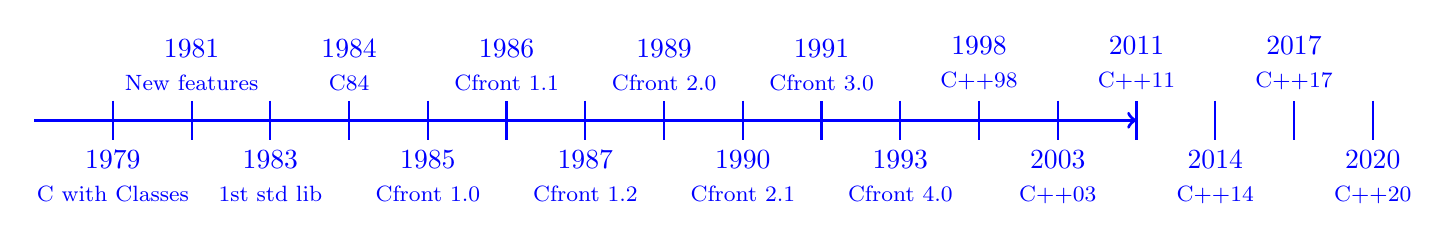
\begin{tikzpicture} 
        \draw[very thick,->,blue] (-1,0)--(13,0); % x axis
        \draw[thick,-,blue]
        (0, 0.25)--(0,-0.25) node[align=center,below] {1979\\ \footnotesize C with Classes} %1/42
        (1,-0.25)--(1, 0.25) node[align=center,above] {1981\\ \footnotesize New features}   %3/42
        (2, 0.25)--(2,-0.25) node[align=center,below] {1983\\ \footnotesize 1st std lib}    %5/42
        (3,-0.25)--(3, 0.25) node[align=center,above] {1984\\ \footnotesize C84}
        (4, 0.25)--(4,-0.25) node[align=center,below] {1985\\ \footnotesize Cfront 1.0}
        (5,-0.25)--(5, 0.25) node[align=center,above] {1986\\ \footnotesize Cfront 1.1}
        (6, 0.25)--(6,-0.25) node[align=center,below] {1987\\ \footnotesize Cfront 1.2}
        (7,-0.25)--(7, 0.25) node[align=center,above] {1989\\ \footnotesize Cfront 2.0}
        (8, 0.25)--(8,-0.25) node[align=center,below] {1990\\ \footnotesize Cfront 2.1}
        (9,-0.25)--(9, 0.25) node[align=center,above] {1991\\ \footnotesize Cfront 3.0}
        (10, 0.25)--(10,-0.25) node[align=center,below] {1993\\ \footnotesize Cfront 4.0}
        (11,-0.25)--(11, 0.25) node[align=center,above] {1998\\ \footnotesize C++98}
        (12, 0.25)--(12,-0.25) node[align=center,below] {2003\\ \footnotesize C++03}
        (13,-0.25)--(13, 0.25) node[align=center,above] {2011\\ \footnotesize C++11}
        (14, 0.25)--(14,-0.25) node[align=center,below] {2014\\ \footnotesize C++14}
        (15,-0.25)--(15, 0.25) node[align=center,above] {2017\\ \footnotesize C++17}
        (16, 0.25)--(16,-0.25) node[align=center,below] {2020\\ \footnotesize C++20};
    

%        \draw[very thick,-,blue] (0,-0.25)--(0,0.25) node[above] {\tiny $1979$}; % y axis
%        \node[red,below] at (0,-0.5) {1979};
%        \draw[thick,-,blue] (1,-0.25)--(1,0.25) node[below] {\small $1989$}; % y axis
%        \node[red,above] at (1,0.5) {1989};
%\draw (0,0) -- (3,1)
%node[pos=0]{0} node[pos=0.5]{1/2} node[pos=0.9]{9/10};
    \end{tikzpicture}
}
